%!TEX root=masterproef.tex

\chapter{Inleiding}
\label{inleiding}

Ofschoon de naam nog geen gemeengoed is, is de opmars van draadloze
sensornetwerken (DSN) in ons dagelijks leven niet meer te stoppen. Na de
revolutie van de persoonlijke computer, de smartphone en het tablet vinden nu
onafhankelijke, minuscule computers hun weg naar allerlei alledaagse dingen en
plaatsen in ons leven. Met hun sensoren kunnen ze de kleinste wijzigingen in
hun omgeving optekenen en via een draadloos netwerk staan ze in verbinding met
elkaar en de buitenwereld. Zo leveren ze hun informatie af, waardoor wij op elk
moment precies weten hoe warm het in elke kamer in ons huis is of welke
groenten we nog in de koelkast hebben liggen. Het lijkt soms nog science
fictie, maar de toekomst is al heel wat dichterbij dan we soms denken.

Indien we deze technologie willen omarmen en ons leven verder willen inrichten
met al deze fantastische ondersteunende hulp, moeten we ons er wel van
vergewissen dat deze technologie betrouwbaar en veilig is. Als enkele sensoren
in ons huis slechts een kleine stap met weinig potenti\"ele, problematische
gevolgen lijkt, moeten we ons misschien toch maar eens bezinnen en beseffen dat
al deze kleine computers met hun sensoren wel eens zeer interessante
mogelijkheden bieden aan anderen met minder positieve bedoelingen.

Misschien wil de concurrent van de producent van onze yoghurt zijn collega wel
in diskrediet brengen door er voor te zorgen dat onze slimme koelkast het
nalaat ons te verwittigen dat het potje yoghurt al een week vervallen is.
Misschien vindt de gasleverancier het wel leuk om overdag, wanneer we niet
thuis zijn, de thermostaat een graadje hoger te zetten. 

De mogelijkheden die draadloze sensornetwerken met zich meebrengen zijn zonder
twijfel fantastisch en ze kunnen de kwaliteit van ons leven ingrijpen
veranderen. Ze mogen echter geen nieuwe bedreiging introduceren. In deze
masterproef duiken we in de wereld van draadloze sensornetwerken en willen we
nagaan of en hoe we deze kunnen voorzien van voldoende bescherming tegen zij
met minder goede bedoelingen.

In dit eerste hoofdstuk introduceren we draadloze sensornetwerken. Hoe zijn ze
opgebouwd? Wat zijn hun mogelijkheden en beperkingen? (\ref{section:wsn}) Wat
zijn de gevaren waaraan ze blootgesteld zijn? Hoe kunnen deze gevaren
vastgesteld worden? Hoe kunnen sensorknopen tegen deze gevaren beschermd
worden? (\ref{section:beveiligen})

Verder defini\"eren we het probleem dat we willen aanpakken
(\ref{section:probleem}) en stellen onze doelstelling voor
(\ref{section:doelstelling}). Na dit hoofdstuk liggen alle speelstukken op
tafel.

\section{Draadloze sensornetwerken}
\label{section:wsn}

Sinds de late jaren '90 zijn draadloze sensornetwerken een bron geweest voor
een explosie aan onderzoek. Binnen en buiten universiteiten werden deze
netwerken ingezet voor allerhande toepassingen: van het opvolgen van
microklimaten bij het telen van gewassen door \cite{baggio2005wireless} tot het
vastleggen van vulkanische activiteit \cite{werner2005monitoring} of het
opvolgen van overstromingsgebieden \cite{hughes2006gridstix}.

Wat moeten we ons eigenlijk voorstellen bij een draadloos sensornetwerk? We
bekijken kort de sensorknopen, waarmee het netwerk wordt opgebouwd. Vervolgens
belichten we het draadloze netwerk dat de knopen in staat stelt om met elkaar
en met de buitenwereld te communiceren.

\subsection{Sensorknopen}

Sensorknopen zijn in essentie zeer eenvoudige computers. Ze worden typisch
opgebouwd rond een microcontroller (\mcu). Dit is een digitaal ontwerp dat
zowel een processor, als geheugen en invoer- en uitvoerkanalen bevat op \'e\'en
enkele ge\"integreerde schakeling. Ze worden daarom ook wel
\emph{systeem-op-een-chip} genoemd. Figuur \ref{fig:motes} toont enkele
typische sensorknopen.

\begin{figure}[ht]
\centering
\begin{subfigure}{.24\textwidth}
  \centering
  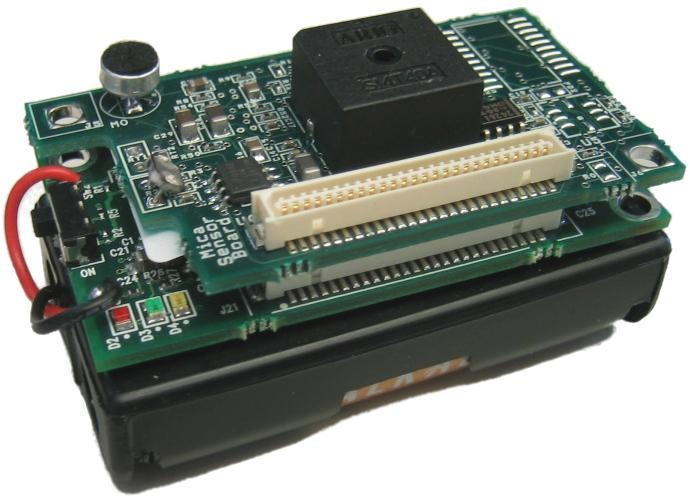
\includegraphics[width=.9\linewidth]{./resources/mica2.jpg}
  \caption{Mica2}
  \label{fig:mica2}
\end{subfigure}
\begin{subfigure}{.24\textwidth}
  \centering
  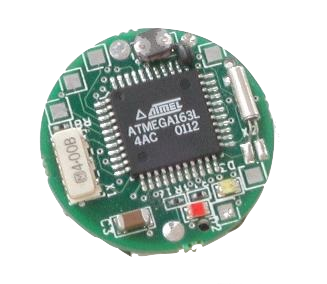
\includegraphics[width=.9\linewidth]{./resources/dot.png}
  \caption{Dot}
  \label{fig:dot}
\end{subfigure}
\begin{subfigure}{.24\textwidth}
  \centering
  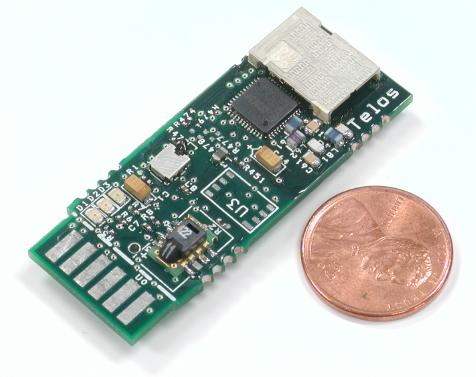
\includegraphics[width=.9\linewidth]{./resources/telos.jpg}
  \caption{Telos}
  \label{fig:telos}
\end{subfigure}
\begin{subfigure}{.24\textwidth}
  \centering
  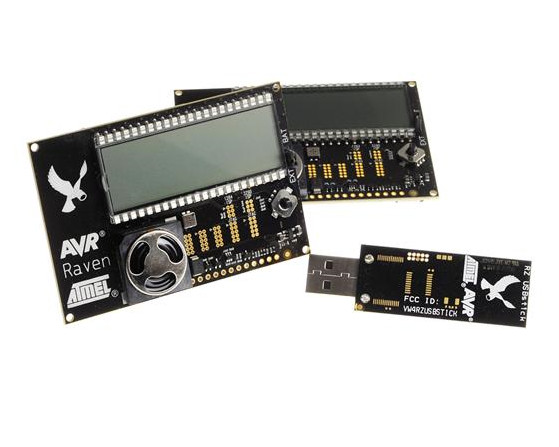
\includegraphics[width=.9\linewidth]{./resources/raven.jpg}
  \caption{AVRraven}
  \label{fig:raven}
\end{subfigure}
\caption{Voorbeelden van sensorknopen.}
\label{fig:motes}
\end{figure}

Naast de \mcu heeft een typische sensorknoop tevens een draadloze radio. Je kan
dit vergelijken met de Wi-Fi verbinding die je tegenwoordig in de meeste
computers of smartphones vindt. Voor sensorknopen wordt echter meestal
geopteerd voor een draadloze radio die een minimum aan energie probeert te
verbruiken. Verschillende nieuwe draadloze netwerkstandaarden zijn de laatste
jaren op het voortouw getreden. De bekendste zijn 6LoWPAN \cite{rfc:6282} en
ZigBee \cite{alliance2012zigbee}. Voor deze masterproef kozen we ZigBee als
technische draadloze standaard. In de volgende paragrafen bekijken we de manier
waarop deze standaard opgebouwd is en werkt, enerzijds omwille van de
toepassing in deze masterproef, maar anderzijds ook wegens de voorbeeldfunctie
die de standaard kan aannemen voor deze groep van draadloze standaarden.

\subsection{ZigBee}
\label{subsection:zigbee}

ZigBee zelf is slechts een laag bovenop de netwerklaag gekend als IEEE 802.15.4
\cite{ieee2009802.15.4}. Deze laag voorziet standaarden op vlak van
energiegebruik, adressering, foutcorrectie, vormgeving van berichten,\dots en
vormt zo de fundamenten voor \emph{low-rate wireless personal area networks}
(LR-WPAN). Bovenop deze laag voegt ZigBee nog drie belangrijke eigenschappen:
routering, ad-hoc netwerk creatie en zelfherstellende maasnetwerken
\cite{oreilly2010buildingwsn}.

Een ZigBee netwerk wordt opgebouwd door knopen die elk \'e\'en van drie
verschillende functies kunnen innemen: co\"ordinator, router of eindknoop. Elk
netwerk heeft precies \'e\'en \emph{co\"ordinator}. Deze knoop is
verantwoordelijk voor het samenbrengen van het netwerk en definieert de
parameters van het netwerk, bv. met betrekking tot de beveiliging.

Een \emph{router} stelt andere knopen in staat om met elkaar te communiceren.
Deze knopen zijn daarom meestal voorzien van een permanente stroomvoorziening,
omdat ze in tegenstelling tot \emph{eindknopen}, zich niet in een slaapstand
kunnen zetten, wegens hun communicatieondersteunende rol.

\emph{Eindknopen}, tot slot, kunnen zich louter verbinden met een netwerk en er
berichten naartoe sturen. Ze kunnen geen berichten van andere knopen voor
andere knopen ontvangen en doorsturen. Typisch trachten ze ook hun
energieverbruik te minimaliseren door hun draadloze radio zoveel mogelijk uit
te schakelen. Hierdoor worden ze onbereikbaar. Het is dankzij de \emph{routers}
die berichten voor de \emph{eindknopen} tijdelijk opslaan, dat deze
\emph{eindknopen} toch alle berichten kunnen ontvangen.

\subsection{Netwerk topologie en adressen}
\label{subsection:topologie}

Met knopen kunnen verschillende netwerk topologie\"en gebouwd worden. Figuur
\ref{fig:topologie} geeft een overzicht van de mogelijkheden. In zijn
eenvoudigste vorm bestaat een netwerk uit een co\"ordinator en een eindknoop.
Wanneer meerdere eindknopen verbonden zijn met dezelfde co\"ordinator, vormen
zij een stertopologie. Alle communicatie verloopt via de centrale
co\"ordinator. In een maasnetwerk, worden routers ingeschakeld om communicatie
via verschillende wegen mogelijk te maken. Eindknopen zijn verbonden met deze
routers of de co\"ordinator, routers en de co\"ordinator kunnen berichten
ontvangen van eindknopen en deze versturen naar andere eindknopen, al dan niet
via andere routers. Een speciale vorm van een maasnetwerk is een clusterboom.
Hierbij vormen groepen van eindknopen en een router een cluster. De router is
verbonden met de co\"ordinator, eventueel opnieuw via andere routers, en zo
wordt een boomstructuur gevormd. De routers die de clusters van eindknopen
realiseren worden ook clusterhoofden genoemd.

\begin{figure}[ht]
  \centering
  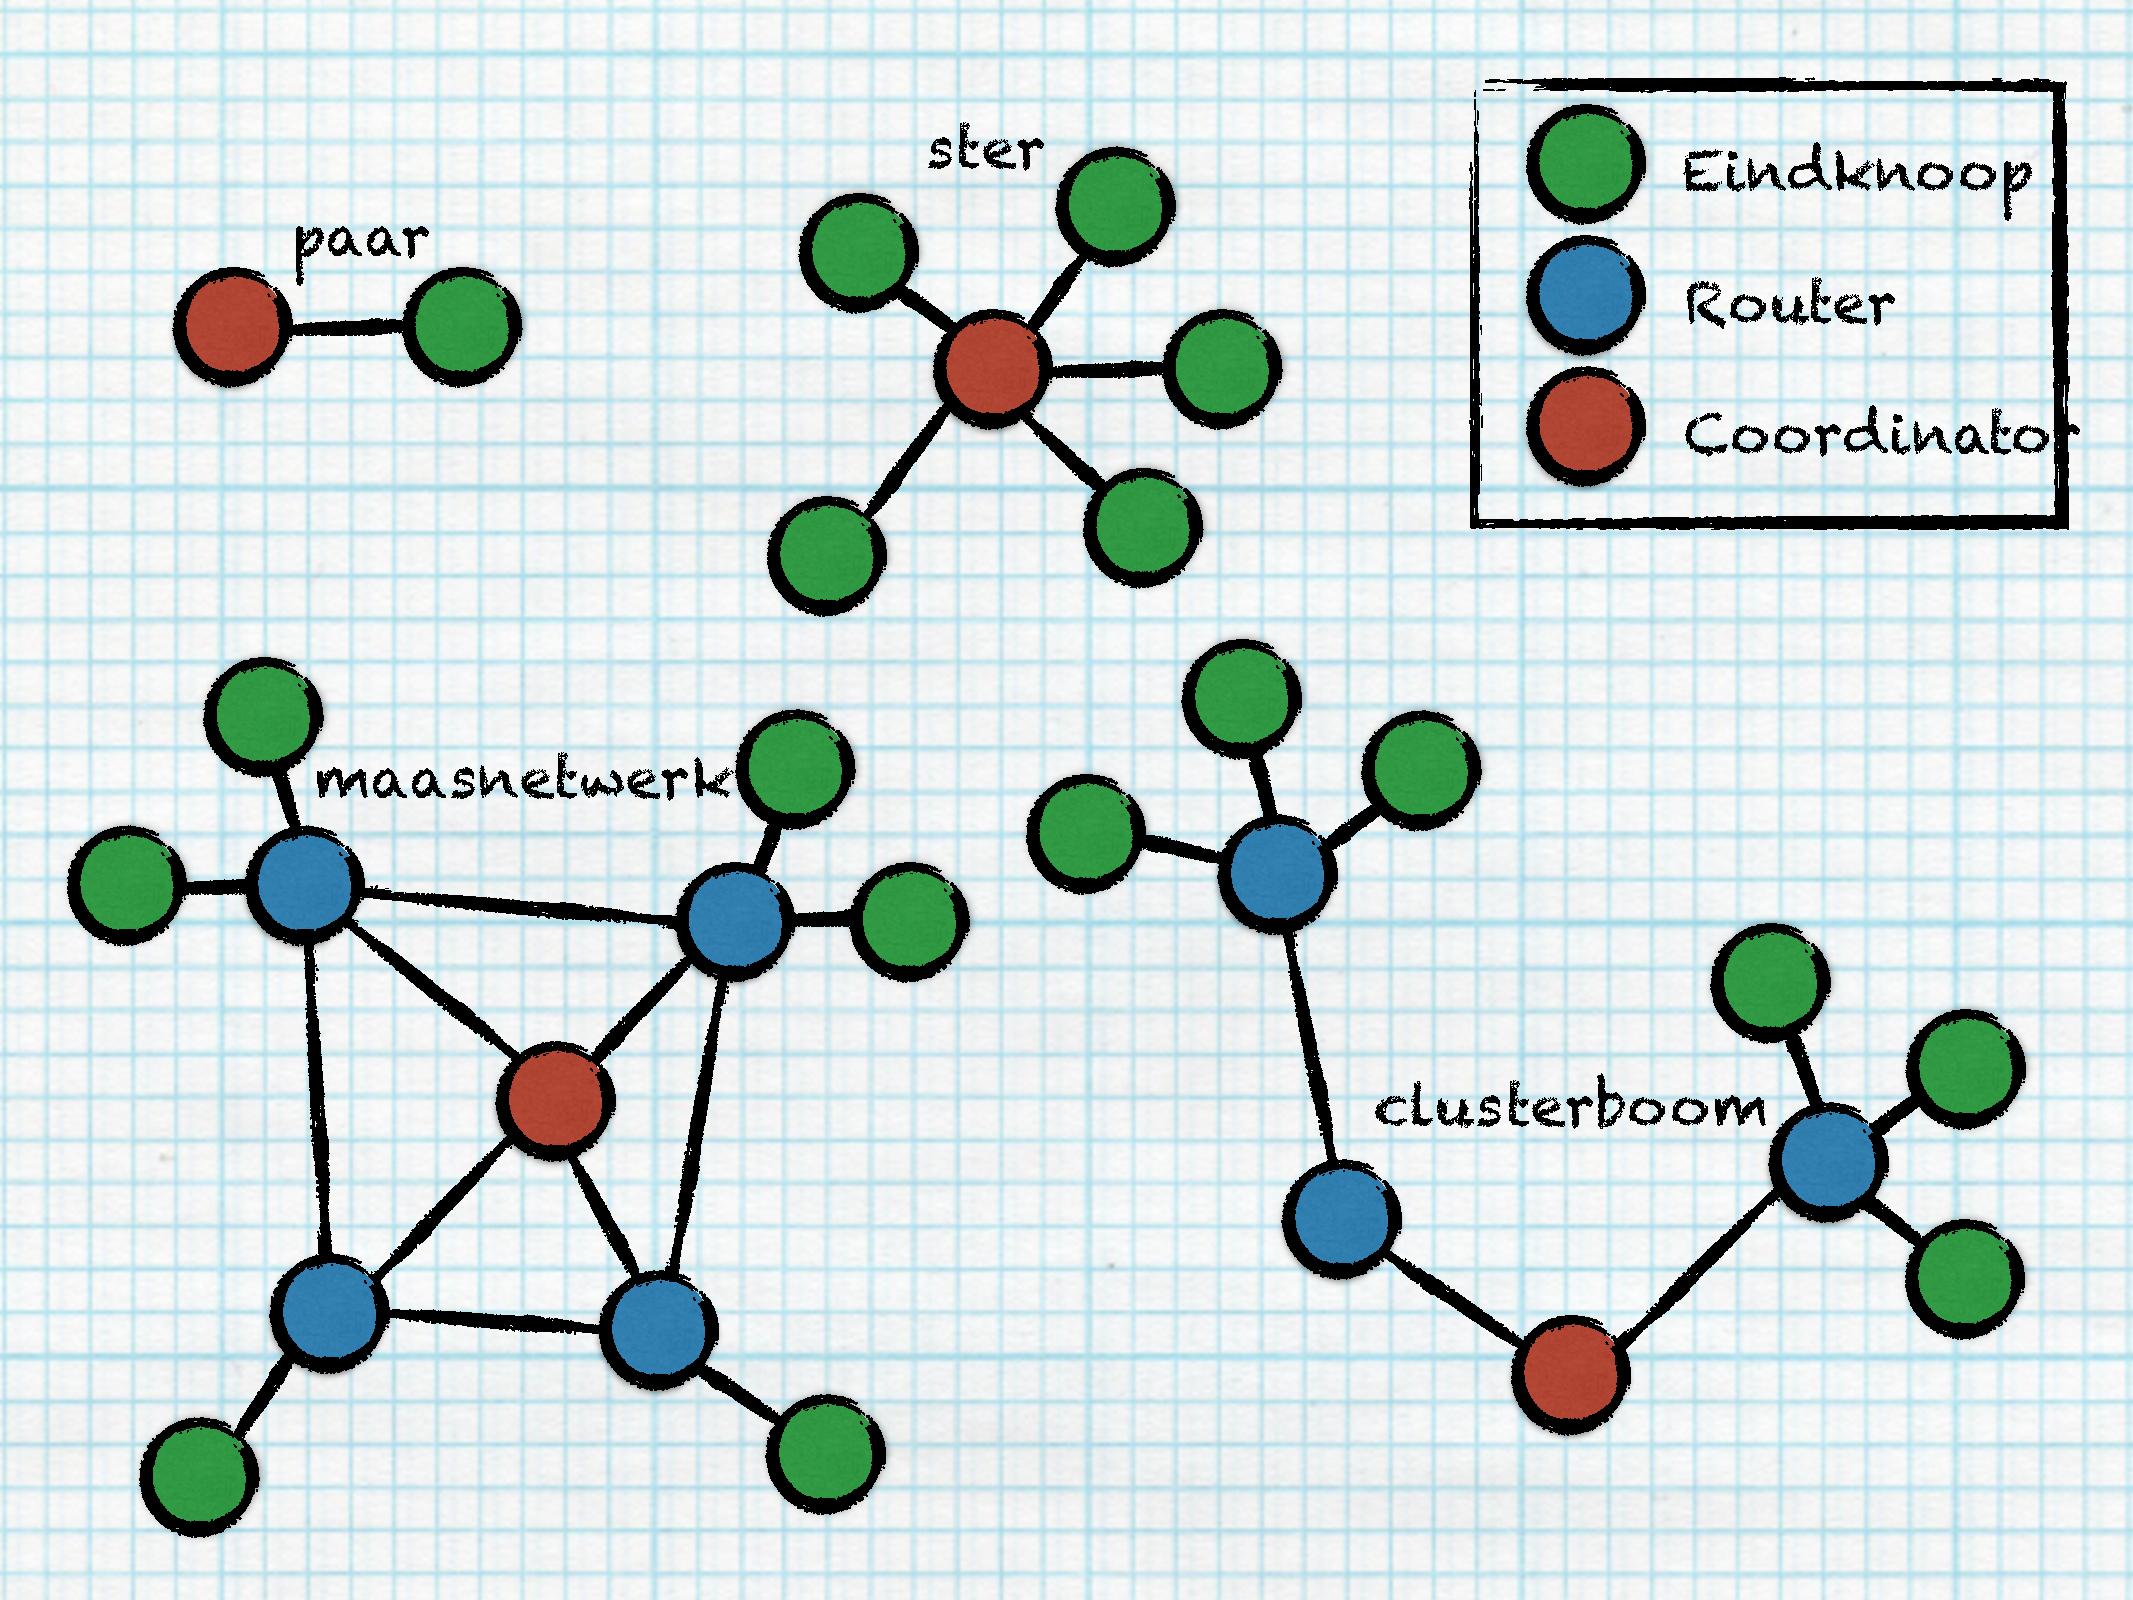
\includegraphics[width=0.7\linewidth]{resources/topology.pdf}
  \caption{Verschillende mogelijke netwerktoplogie\"en.}
  \label{fig:topologie}
\end{figure}

Het lijkt evident, maar elke knoop, in eender welke topologie, heeft een eigen,
uniek adres. Eigenlijk meerdere. Zo heeft een ZigBee knoop een uniek adres
binnen het netwerk waaraan het deelneemt. Dit adres wordt door de co\"ordinator
van het netwerk toegekend aan een knoop wanneer deze toetreedt tot het netwerk.
Dit \emph{netwerk adres} bestaat uit 16 bits en laat dus toe om 65534
verschillende adressen toe te kennen. Het adres \ttt{0x0000}\footnote{We
hanteren voor de notatie van adressen de hexadecimale voorstelling. Elk cijfer
stelt een groep van 4 bits voor. 4 groepen stellen zo een 16 bit adres voor.}
reserveert de co\"ordinator voor zichzelf en het adres \ttt{0xFFFE} wordt
typisch gebruikt als het zgn. \emph{broadcast adres}, het adres waarnaar een
bericht gestuurd wordt dat bij alle andere knopen dient afgeleverd te worden.

Maar daarnaast heeft elke ZigBee radio ook een eigen, unieke adres dat
gegarandeerd overal uniek is. Dit adres bestaat uit 64 bits en wordt
samengesteld uit een hoog en laag gedeelte. Het hoge gedeelte beslaat de eerste
32 bits en is voorbehouden voor de unieke identificatie van de producent van de
radio. De lage reeks van 32 bits is een uniek nummer binnen de productie van de
producent. Het is daarom logisch dat er gebruik gemaakt wordt van een
\emph{netwerk adres}, dat slechts 16 bits groot is en dus een aanzienlijke
besparing aan geheugen kan opleveren.

Naast de adressen van de knopen is er ook nog het zogenaamde \emph{personal
area network (PAN)} adres. Dit is een unieke identificatie van het netwerk dat
door de co\"ordinator georganiseerd wordt. Ook dit is een 16 bit adres en laat
dus toe om 65536 netwerken op te bouwen.

Tot slot kunnen ZigBee radio's ook gebruik maken van 12 verschillende kanalen,
zodat de volledige adresstructuur bestaat uit een kanaal, een PAN adres en een
netwerk adres.

\section{Beveiligen van sensorknopen}
\label{section:beveiligen}

Het beveiligen van sensorknopen is in tegenstelling tot de beveiliging van
klassieke computers een bijzonder moeilijke aangelegenheid. De computers waar
onze emails, foto's en andere kostbare documenten opgeslagen zijn, zijn
uitgerust met een virusscanner, firewall,\dots. Dit is mogelijk omdat ze
voorzien zijn van een constante stroomvoorziening. Ze zijn tevens beschermd
door ons huis of het datacenter van onze leverancier van internetdiensten.

In \cite{dargie2010fundamentals} wordt een goed overzicht gegeven van de
uitdagingen die het beveiligen van DSN met zich meebrengen, in tegenstelling
tot de klassieke situatie. Een sensorknoop heeft geen constante
stroomvoorziening en moet het veelal stellen met een zeer beperkte batterij.
Verder ligt de sensorknoop meestal letterlijk \emph{ten velde} en is fysiek
toegankelijk voor nagenoeg iedereen.

Verder is er geen centraal punt waar alle communicatie van en naar de
sensorknoop gegarandeerd passeert. Het enige communicatiemedium is het
draadloze netwerk en via die weg kan men steeds rechtstreeks contact leggen met
elke afzonderlijke knoop, zonder dat een andere knoop dit ooit merkt. Tot slot
is het belangrijk dit nog aan te vullen met het feit dat een draadloos
communicatiemedium inherent fouten met zich meebrengt, en dat berichte verloren
kunnen gaan.

\subsection{CIA, AAA en andere beveiligingsprincipes}
\label{subsection:cia}

Beveiliging is een zeer ruim begrip dat veel aspecten onder zijn vleugels
draagt. Het is belangrijk deze waaier voor ogen te houden wanneer we
beveiliging bespreken. Wanneer men spreekt over het beveiligen van computers en
netwerken, wordt dikwijls gerefereerd naar het CIA beveiligingsmodel. Dit
letterwoord staat voor: vertrouwelijkheid (Engels: \emph{confidentiality}),
integriteit en beschikbaarheid (Engels: \emph{availability}).

Om \emph{vertrouwelijkheid} te garanderen moet beveiliging de nodige
voorzieningen treffen om er voor te zorgen dat bv. een bericht enkel door de
bedoelde bestemmeling kan begrepen worden. Onder \emph{integriteit} verstaat
men het principe dat dat bericht dan weer niet mag gewijzigd kunnen worden, of
dat de bedoelde bestemmeling van het bericht ten minste kan valideren dat er
aan het bericht niets gewijzigd is. Maar beveiliging moet ook de
\emph{beschikbaarheid} van onderdelen van het netwerk garanderen, om er zeker
van te zijn dit laatste zijn diensten kan blijven aanbieden.

Het CIA model is zonder meer een belangrijke basis, maar er ontbreken nog veel
belangrijke aspecten. In \cite{rfc:3198} wordt een gestandaardiseerde
terminologie voorgesteld voor het defini\"eren van een beveiligingsbeleid.
Naast de drie hoofdpijlers van het CIA model vinden we zo ook nog een ander
belangrijk model, namelijk het AAA (Engels: \emph{triple A}): authenticatie,
autorisatie en vaststellen (Engels: \emph{accounting})

Via \emph{authenticatie} kan de identiteit van een gebruiker of apparaat
vastgesteld worden, zodat eenduidig kan bepaald worden van wie bv. een bericht
in het netwerk komt. \emph{Autorisatie} is daarentegen het proces waarbij
nagegaan wordt of een gebruiker waarvan de authenticiteit is vastgesteld, een
bepaalde handeling \emph{mag} uitvoeren. Ten slotte biedt het
\emph{vaststellen} van alle gebeurtenissen en beslissingen binnen het
beveiligde domein, een belangrijke bron van informatie om een beleid verder te
verfijnen en eventueel bij te sturen.

In het kader van beveiliging wordt typisch ook gesproken over een \emph{beleid}
(Engels: \emph{policy}), waarin de regels waaraan alle spelers binnen het te
beveiligen domein zich aan dienen te houden of moeten aan gehouden worden.
Componenten zoals een \emph{policy decision point} (PDP) en een \emph{policy
enforcement point} (PEP) worden tevens ge\"introduceerd om respectievelijk de
verantwoordelijkheid voor het beslissen op basis van en uitvoeren van deze
beslissingen volgens het beleid aan te duiden.

Naast deze zes aspecten, is er ook nog het principe van onweerlegbaarheid
(Engels: \emph{nonrepudiation}). Door garanties omtrent
\emph{onweerlegbaarheid} in te bouwen, kan bv. een ontvanger er zeker van zijn
dat een zender van een bericht effectief dit bericht verstuurd heeft.

Een aantal gekende technieken bieden klassiek oplossingen voor verschillende
van de hoger vermelde principes: Digitale handtekeningen kunnen helpen bij het
garanderen van de \emph{authenticiteit}, \emph{onweerlegbaarheid} en
\emph{integriteit} van een boodschap. Cryptografie kan logischerwijs de
\emph{vertrouwelijkheid} van berichten garanderen, maar kan ook aan de hand van
publieke en private sleutels de \emph{authenticiteit} bevestigen, omdat
berichten slechts kunnen versleuteld worden met de overeenkomstige sleutel van
het paar.

In hoofdstuk \ref{chapter:achtergrond} gaan we dieper in op de typische
eigenschappen van sensorknopen en belichten we tal van beveiligingsrisico's
waaraan DSN blootgesteld zijn. Aan de hand van de zonet beschreven principes
zullen we zien dat DSN inherent moeilijk te beveiligen zijn en dat het nagenoeg
onmogelijk is om inbraken te verijdelen.

\subsection{Inbraakdetectie}
\label{subsection:detection}

Indien het verijdelen van inbraken nagenoeg onmogelijk is, moet een belangrijke
tweede beveiligingslinie opgetrokken worden: inbraakdetectie.

Indien we niet weten dat een inbraak heeft plaatsgevonden, zullen we enkel
berusten in een vals gevoel van veiligheid. Het is niet omdat we het niet weten
dat er inbraakpogingen zijn, dat ze er effectief niet zijn. Misschien moeten we
zelfs durven stellen dat het belangrijk is om meer te weten dan te verijdelen,
omdat het tweede in essentie berust op de kennis van het eerste.

Inbraakdetectie is typisch de stille vennoot in een beveiligingsverhaal. Daar
waar bv. een firewall of authenticatie server actieve toegang ontzegt, zal een
inbraakdetectiesysteem (IDS) typisch geen actieve rol spelen\footnote{Er zijn
wel degelijk toepassingen waarbij een IDS informatie kan verschaffen aan bv.
een firewall. Indien het IDS een inbraakpoging detecteert kan de oorsprong van
de inbraakpoging door de firewall gebruikt worden om op netwerkniveau toegang
tot het netwerk te ontzeggen.}. Het IDS zal eerder bewijsmateriaal verzamelen
om een inbraakpoging degelijk te documenteren. Uit deze informatie kunnen dan
bijsturingen aan het beleid aangebracht worden, waardoor de actieve componenten
in de toekomst wel in staat zijn om eventueel inbraakpogingen van die aard te
verijdelen.

Deze architectuur legt al snel een belangrijk pijnpunt bloot: in een klassiek
netwerk wordt het netwerk beschermd aan de buitenzijde. De firewall schermt het
interne netwerk af van aanvallen van buiten het netwerk. Als een
spreekwoordelijke muur van vuur wordt elke toegang tot het netwerk gelouterd en
\emph{slechte berichten} worden onherroepelijk verbrand voor ze het netwerk
kunnen betreden.

Het IDS wordt daarom typisch ook op het interne netwerk aangesloten daar waar
alle netwerkverkeer dat door de firewall wordt doorgelaten passeert. Alle
aanvallen die toch nog door de firewall zijn kunnen geraken, kunnen dan door
het IDS gedetecteerd worden.

Dit lijkt op het eerste zicht een vreemde tegenspraak. Indien het IDS deze
aanvallen eventueel kan detecteren, waarom wordt deze kennis dan niet gebruikt
op het niveau van de firewall? De reden ligt in de natuur van de firewall. Deze
werkt immers hoofdzakelijk op netwerk niveau en bekijken elk netwerkpakket op
zich. Aanvallen zijn soms een samengang van verschillende van zulke pakketten
en typisch zelf eerder van pakketten die op zich perfect legaal zijn. Het
draait hier hoofdzakelijk om de inhoud van de pakketten en de analyse vraagt
een kennis van de toepassingen waarmee gecommuniceerd wordt. Soms kan zelfs
slechts aan de inhoud van antwoorden uit het interne netwerk opgemaakt worden
dat er een inbraak plaatsgevonden heeft. Deze complexiteit is te groot om op
het niveau van een firewall degelijk te realiseren.

De resultaten van een IDS zullen dikwijls eerder leiden tot verbeteringen aan
de toepassingen binnen het interne netwerk, zodat deze niet meer vatbaar zijn
voor het soort inbraken dat gedetecteerd werd.

Wanneer we dit nu afspiegelen op een DSN, merken we al snel dat hier enkele
fundamentele principes zulk een architectuur onmogelijk maken: een DSN heeft
geen afgebakende netwerkrand, er is geen uniek punt waar alle netwerkverkeer
langs passeert en waar een firewall zou kunnen ge\"introduceerd worden, laat
staan dat er een manier zou zijn om al het interne verkeer op \'e\'en enkele
plaats te analyseren.

Binnen een DSN is het letterlijke elke knoop voor zichzelf: elke knoop kan
immers van buitenaf benaderd worden zonder te moeten passeren langs een
gemeenschappelijk controlepunt.

\section{Probleemstelling}
\label{section:probleem}

DSN en sensorknopen op zich zijn duidelijk geen makkelijke klanten wanneer het
beveiliging betreft. Enerzijds hebben ze nagenoeg onvoldoende middellen om zich
te beschermen en anderzijds is hun situatie zo dat het letterlijk elke knoop
voor zichzelf is en dat ze nauwelijks kunnen vertrouwen op hun collega knopen.

In dit kader eisen wij, de gebruikers van het DSN, toch dat er voldoende
garanties worden gegeven zodat we ons voldoende verzekerd voelen om onze meest
intieme informatie toe te vertrouwen aan deze netwerken.

Aangezien het haast onmogelijk is om inbraakpogingen te verijdelen is het van
groot belang dat we in staat zijn ze ten minste vast te stellen. Het
introduceren van een IDS in het DSN is dan weer een directe aanval op de
essenti\"ele functionaliteit van een sensorknoop, waardoor de mogelijkheden
sterk beperkt worden.

\section{Doelstelling}
\label{section:doelstelling}

Zoals we zullen zien in sectie \ref{section:related}, ligt in de literatuur
betreffende ``inbraakdetectie in draadloze sensornetwerken'' de nadruk in
hoofdzaak op het detecteren van specifieke aanvallen of het vaststellen van
anomalie\"en in het verwachte gedrag van sensorknopen en/of het netwerk dat hen
verbindt.

Deze werken stellen tevens dat het een nagenoeg onmogelijke taak is om alle
benodigde detectiemechanismen effectief te implementeren. Dit is logisch
gegeven het beperkte aanbod aan middelen die sensorknopen typisch ter hunnen
beschikking hebben. Zo zou bv. een exhaustieve lijst van aanvalspatronen
slechts in sensorknopen met zeer grote hoeveelheden geheugen kunnen opgeslagen
worden en zouden de berekeningen die nodig zijn om verschillende anomalie\"en
te detecteren gewoonweg te veel energie verbruiken.

Als in deze fase van onderzoek naar systemen om inbraken te detecteren het niet
mogelijk is om een sluitend IDS voor DSN te ambi\"eren, lijkt het opportuun om
een stap terug te nemen en de focus te leggen op de middelen die nodig zijn om
de reeds beschreven en mogelijk ook toekomstige oplossingen te realiseren. Is
het mogelijk om een raamwerk te cre\"eren dat een ontwikkelaar van een
sensorknoop in staat stelt om een selectie van de in de literatuur beschreven
oplossingen te implementeren, zonder een diepgaande analyse van de
onderzoeksliteratuur en zonder zich zorgen te moeten maken over de
onderliggende interactie met andere knopen, het vergaren en opvragen van
informatie op systeem-niveau,\dots?

Deze thesis wil zulk een raamwerk ontwerpen, implementeren en de impact ervan
bepalen. Daartoe zal eerst een lijst gemaakt worden van de verwerkte
oplossingen, waaruit de functionele en technische vereisten voor het raamwerk
gedistilleerd kunnen worden. Vervolgens zal een architectuur voorgesteld worden
die aan deze vereisten voldoet. Aan de hand van een implementatie van deze
architectuur zal tot slot nagegaan worden wat de impact is van dit raamwerk met
betrekking tot geheugen en rekenkracht.

De voordelen van zulk een raamwerk zijn legio: een herbruikbaar raamwerk neemt
zorgen, gemeenschappelijk aan de verschillende oplossingen weg en kan zorgen
voor een optimale implementatie. Door middel van een goedgekozen technische
architectuur kan tevens platform-onafhankelijheid nagestreefd worden.
